\subchapter{Setting up the serial communication}
{Objective: Get a working serial communication for the console}

After this lab, you will be able to communicate with your \devboard over the console

\section{Install the picocom program}

If you did not run \code{make prepare} in \labdir, you need to install \code{picocom} now.

The code below will install \code{picocom} and make your user belong to the \code{dialout} 
group, which is needed for you to be allowed to write to the serial console:

Alternatively:

\begin{verbatim}
sudo apt-get install picocom
sudo adduser ${USER} dialout
\end{verbatim}

You need to log out and in again for the group change to be effective.

\section{Setting up serial communication with the board}

Make sure that the USB-to-Serial cable to the \devboard is disconnected from your computer. Check that no other USB serial ports are connected to the system

{\small
{\tt
ls /dev/ttyU*
}
}

Plug the \devboard into your computer using the provided
USB-to-serial cable. When plugged-in, a serial port should appear as
\code{/dev/ttyUSB0} if there are no other USB - Serial ports.
Otherwise find out which serial port was just activated using \code{dmesg}

{
  \begin{center}
    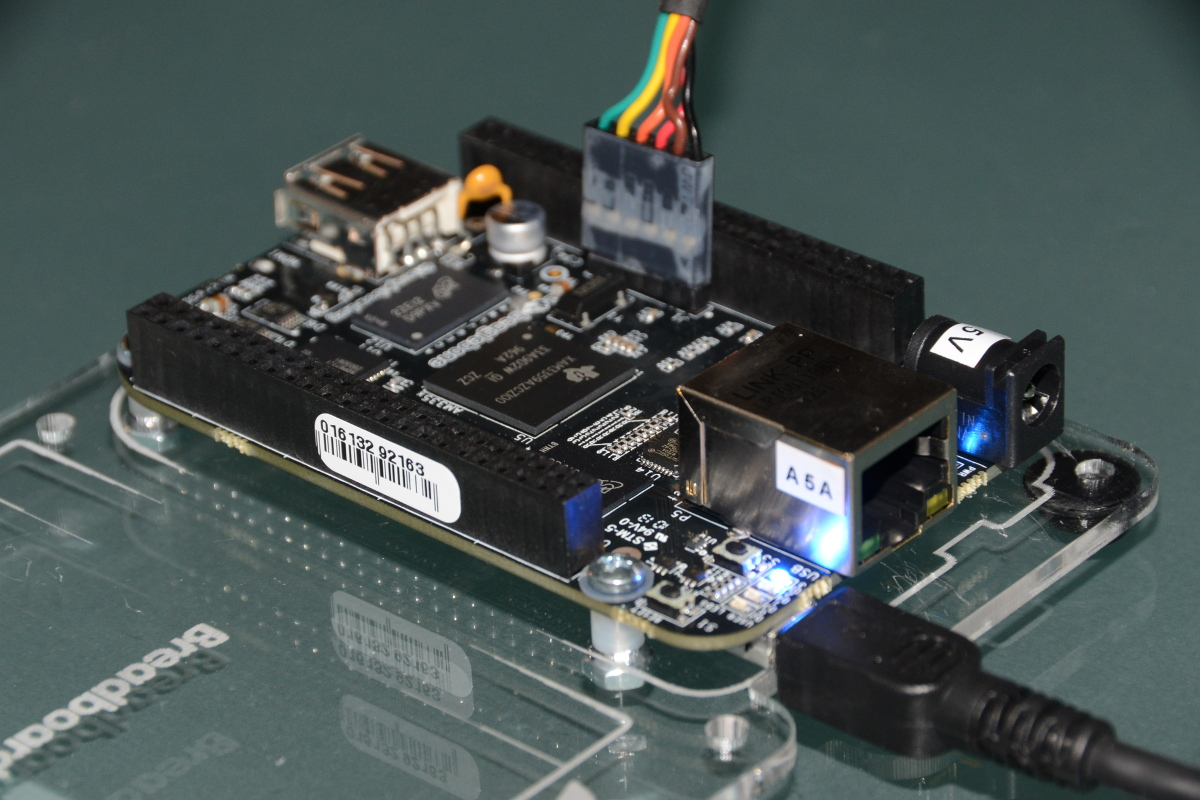
\includegraphics[height=5cm]{labs/setup-serial/beaglebone-black-serial.jpg}
  \end{center}
}

You can also see this device appear by looking at the output of
\code{dmesg}.



Run \code{picocom -b 115200 /dev/ttyUSB0}

to start serial communication on \code{/dev/ttyUSB0}, with a baudrate of 115200.

If you wish to exit \code{picocom}, press \code{[Ctrl][a]} followed by
\code{[Ctrl][x]}.

